\documentclass[a4paper,12pt]{report}
\usepackage[utf8]{inputenc}
\usepackage[ngerman]{babel}
\usepackage{titlesec}
\usepackage{graphicx}
\graphicspath{ {./images/} }
\usepackage{setspace}
\usepackage{lipsum}
\usepackage{geometry}
\usepackage{tocbibind}
\usepackage{hyperref}
\usepackage{array}
\usepackage{footnote}
\usepackage{natbib}
\usepackage{listings}
\usepackage{xcolor}
\bibliographystyle{unsrtnat}
\newcommand{\footcite}[1]{\footnotemark\footnotetext{\cite{#1}}}

\renewcommand{\lstlistingname}{Code Snippet}
\lstdefinestyle{codeStyle}{
  language=Java, 
  basicstyle=\ttfamily\small,
  numbers=left,
  numberstyle=\tiny\color{gray},
  stepnumber=1,
  numbersep=5pt,
  showspaces=false,
  showstringspaces=false,
  showtabs=false,
  tabsize=2,
  breaklines=true,
  breakatwhitespace=true,
  stringstyle=\color{red},
  keywordstyle=\color{blue},
  commentstyle=\color{green},
  frame=single,
  rulecolor=\color{gray},
  captionpos=b,
  escapeinside={\%*}{*)},
}





\geometry{a4paper, left=25mm, right=25mm, top=30mm, bottom=30mm}

\titleformat{\chapter}{\normalfont\huge}{\thechapter.}{20pt}{\huge\bfseries}
\titleformat{\section}{\normalfont\Large}{\thesection}{12pt}{\Large\bfseries}
\titleformat{\subsection}{\normalfont\large}{\thesubsection}{8pt}{\large\bfseries}

\title{Webbasierte Multiplayer Schach-App}
\author{Jasper Paul Fülle}
\date{24. Mai 2023}

\begin{document}

\begin{titlepage}
    \begin{center}
        \vspace*{1cm}
        
        \Large
        \textbf{Webbasierte Multiplayer Schach-App}
        
        \vspace{0.5cm}
        
        Bachelorarbeit
        
        \vspace{1.5cm}
        
        \normalsize
        vorgelegt von\\
        Jasper Paul Fülle\\
        Matrikelnummer 3367654
        
        \vspace{1cm}
        
        Betreut von\\
        Prof. Dr. Thorsten Thormälen
        
        \vspace{1cm}
        
        \begin{tabular}{>{\raggedright}p{4cm}>{\raggedleft}p{4cm}}
        Studiengang & Wirtschaftsinformatik \\
        \end{tabular}
        
        \vspace{1cm}
        
        \today
        
        \vfill
        
        
        \vspace{0.5cm}
        
        Fachbereich Mathematik und Informatik\\
        Philipps Universität Marburg
    \end{center}
\end{titlepage}

\tableofcontents

\chapter{Einleitung}
    \section{Motivation}
    Schach ist ein traditionsreiches und abwechslungsreiches Brettspiel, deren Ursprung nicht genau bestimmt werden kann. Es wird vermutet, dass das erste schachähnliche Spiel  \textit{Tschaturanga} seinen Ursprung in Nordindien um 600 n. Chr. hatte\footcite{schachgeschichte}.
    Im Laufe der Jahrhunderte hat Schach eine bedeutende Rolle in der Kultur und Geschichte gespielt. So wurde beispielsweise die Schach-WM 1972 eine Art Machtkampf im kalten Krieg zwischen der UdSSR, welche den damaligen Schach dominierten, und der USA\footcite{bobby}.
    Schach bleibt bis heute ein beliebtes Spiel, welches 2020 durch die Netflix Serie \textit{Damengambit} und 2022 durch den Betrugsvorwurf von Magnus Carlsen an seinen 19-jährigen Gegner Hans Niemann\footcite{schachskandal} eine breitere Aufmerksamkeit erhielt (siehe Abbildung \ref{fig:Schachinteresse}). 
     Darüber hinaus hat Schach im digitalen Zeitalter eine neue Popularität erreicht. Online-Schachplattformen wie \url{chess.com} verzeichnen Milliarden von Live-Partien\footcite{chesscom3}, während Schach Live-Streams auf Plattformen wie \url{twitch.com} Millionen von Followern anziehen.
     
Die Entwicklung einer webbasierten Multiplayer-Schach-App bietet eine einzigartige Gelegenheit, ein traditionsreiches und beliebtes Spiel im digitale Zeitalter weiter zu entwickeln. Meine Motivation für diese Arbeit besteht darin, eine App zu entwickeln, die die Grundlagen einer Schach-App enthält und gleichzeitig eine solide Basis für zukünftige Erweiterungen und Verbesserungen bietet. Insbesondere plane ich, innovative Funktionen zu integrieren, die bislang in den gängigen Schach-Apps nicht vorhanden sind, wie z.B. die Möglichkeit, unterschiedliche Schachfiguren und -bretter als Belohnungen freizuschalten oder mit Freunden eine Gruppe zu gründen, welche in einer Liga auf- und absteigen kann. Durch die Entwicklung einer Schach-App mit neuen Funktionalitäten kann ich dazu beitragen, die Popularität von Schach zu steigern und vor allem das Spiel einem breiteren Publikum zugänglich zu machen.
    \section{Zielsetzung}
    Diese Bachelorarbeit hat das Ziel eine Schach-App zu entwerfen und zu implementieren, die eine intuitive User Experience und ein ansprechendes User Interface mit vielen nützlichen Funktionen beinhaltet.
    
    User Experience (\textit{UX}) bezieht sich darauf wie ein Nutzer sich auf einer Anwendung bewegt und wie einfach und angenehm es für den Nutzer ist, die Funktionen der Anwendung zu verwenden.
    
    Das User Interface (\textit{UI}) beschäftigt sich mit der visuellen und interaktiven Gestaltung von Benutzeroberflächen. Es umfasst die Gestaltung von Buttons, Formularen und anderen visuellen Komponenten, sowie das Feedback dieser Komponenten, wie zum Beispiel die Rückmeldung eines fehlgeschlagenen Logins.
    Zusammengefasst beschäftigt sich UX damit, wie man eine Anwendung verwendet und UI damit, wie die Benutzeroberfläche der Anwendung aussieht.\footcite{webdesign}
        
        Funktionen der Schach-App sind unter anderem das Registrieren und Einloggen, das Versenden, Annehmen und Ablehnen von Freundschaftsanfragen, das Zuschauen bei laufenden Spielen, das Herausfordern von Freunden zu Schachspielen und natürlich das Spielen von Schachpartien mit einem Chat und verschiedenen Einstellungsmöglichkeiten der Schach Uhren selbst.
    Dabei wird besonderer Wert auf die Verwendung moderner Web-Technologien wie React, Node.js, Socket.IO, Redis und PostgeSQL gelegt, um eine optimale Benutzererfahrung und Skalierbarkeit zu gewährleisten. Darüber hinaus soll die Arbeit einen Überblick über die technischen Herausforderungen und Lösungen im Zusammenhang mit der Implementierung einer solchen Schach-App bieten.
    
    \section{Aufbau der Arbeit}
Diese Bachelorarbeit gliedert sich in sechs Hauptkapitel, die jeweils unterschiedliche Aspekte der Entwicklung und Implementierung der Schach-App behandeln.

Im ersten Kapitel, der \textit{Einleitung}, werden die Motivation für die Entwicklung der Schach-App, die Zielsetzung der Arbeit und der Aufbau der Arbeit selbst vorgestellt.

Das zweite Kapitel, \textit{Theoretische Grundlagen}, erläutert die Grundlagen von Schach als Spiel sowie die verwendeten Web-Technologien wie Node.js, Express, Socket.io, React und PostgreSQL, die für das Verständnis der nachfolgenden Kapitel wichtig sind.

Im dritten Kapitel, \textit{Systemarchitektur}, wird die Gesamtarchitektur der Schach-App beschrieben, einschließlich der Unterteilung in Frontend und Backend, der Datenbankstruktur und der Kommunikation zwischen den verschiedenen Komponenten.

Das vierte Kapitel, \textit{Implementierung}, geht auf die praktische Umsetzung der Schach-App ein, indem es die Entwicklungsprozesse für das Frontend und das Backend sowie die Integration der Datenbanken erläutert.

Das fünfte Kapitel, \textit{Tests und Evaluation}, behandelt die verschiedenen Tests, die durchgeführt wurden, um die Funktionalität, Usability, Performance und Sicherheit der Schach-App zu bewerten.

Im abschließenden sechsten Kapitel, \textit{Fazit und Ausblick}, werden die Ergebnisse der Arbeit zusammengefasst, eventuelle Limitationen diskutiert und mögliche Erweiterungen und Weiterentwicklungen für die Schach-App vorgeschlagen.

Die Arbeit endet mit dem \textit{Anhang}, der zusätzliche Grafiken und die Liste der verwendeten Literatur enthält.
\chapter{Theoretische Grundlagen}
    \section{Schach}
   Schach ist ein strategisches Brettspiel für zwei Spieler, welches auf einem quadratischen Spielfeld mit 64 Feldern gespielt wird. Jeder Spieler beginnt mit 16 Figuren und das Ziel des Spiels ist es, den König des Gegners schachmatt zu setzen, indem man ihn bedroht, ohne dass der Gegner den Angriff verhindern kann. 
   
   Wie sich welche Figuren bewegen und andere Figuren schlagen erkläre ich nicht explizit, lediglich zwei Sonderregeln des Schachs werde ich genauer erklären, da diese bei der Umsetzung des Spiels gesondert gehandhabt werden müssen.
   
   Die erste ist das so genannte \textit{en passant}-Regel. Dabei ist es einem Bauern möglich einen gegnerischen Bauer diagonal zu schlagen, falls dieser zwei Felder gezogen ist und nun auf der gleichen Höhe wie der eigene Bauer steht (siehe Abbildung \ref{fig:en-passant}).
   
   Die zweite Zusatzregel ist die \textit{Bauernumwandlung}. Sie besagt, dass falls ein Bauer die gegnerische Grundreihe erreicht, dieser Bauer in eine Dame, einen Springer, einen Turm oder einen Läufer umgewandelt werden kann (siehe Abbildung \ref{fig:promotion}).
    \section{Web-Technologien}
        \subsection{Node.js und Express}
        \subsubsection{Node.js und seine Vorteile}
Node.js ist eine JavaScript-Laufzeitumgebung, welche erstmals 2009 angekündigt wurde\footcite{nodeyoutube} und speziell für die Entwicklung von skalierbaren Netzwerkanwendungen entworfen wurde\footcite{nodejs}. Skalierbarkeit bedeutet, dass mit steigender Benutzeranzahl der Ressourcenverbrauch idealerweise linear steigt. Zu den relevanten Ressourcen von Webanwendungen gehören Rechenleistung, Ein-/Ausgabeoperationen (\textit{I/O}) und Arbeitsspeicher, wobei Node.js vor allem die Skalierbarkeit von I/O intensiven Anwendungen verbessert\footcite{nodejsbook}.
I/O-Zugriffe sind beispielsweise Zugriffe auf Datenbanken, Webservices oder auf das Dateisystem. Node.js setzt dabei vollständig auf asynchrone Zugriffe. Dabei wartet der Thread nicht auf das Ergebnis eines I/O-Zugriffs, sondern führt andere Aufgaben aus, bis das Ergebnis verfügbar ist. Anschließend wird eine zuvor definierte Callback Funktion (siehe Code Snippet \ref{lst:callback}) durchgeführt. Bei einem synchronen Zugriff, wie es bei einigen anderen Laufzeitumgebungen der Fall ist, würde der Thread auf das Ergebnis warten und dieses anschließend weiterverarbeiten, wobei jedoch sein Speicherplatz zum Teil belegt bleibt. Die Vorteile hinsichtlich der Skalierbarkeit werden jedoch erst bei einer hohen Anzahl von Zugriffen erkennbar.

\begin{lstlisting}[style=codeStyle, caption={Beispiel einer Callback Funktion \textbf{Quelle: } \cite{nodejsbook}}, label={lst:callback}]
database.query(  "SELECT * FROM user",  function(result) {
result...
});
\end{lstlisting}


Ein für mich großer und entscheidender Vorteil der Nutzung von Node.js ist, ist die Nutzung der gleichen Programmiersprache für Frontend und Backend, zumal die Syntax von JavaScript mir auch schon ein wenig geläufig war.
In einem Team-Projekt kann das natürlich besonders nützlich sein, da Kommunikationsbarrieren durch unterschiedliche Programmiersprachen von Frontend und Backend niedriger sind. Natürlich versteht deshalb der Frontend-Entwickler nicht alles was  der Backend-Entwickler macht und umgekehrt, jedoch gibt es eine gemeinsame Grundlage. Neben den Kommunikationsvorteilen ermöglicht die Verwendung von der gleichen Programmiersprache im Frontend und Backend das Teilen von Code. So ist es zum Beispiel möglich Callback Funktionen vom Frontend an das Backend zu senden und dort aufzurufen.

Node.js basiert auf der Verarbeitung von Requests vom Frontend und dem zurück senden von einem Result mittels dem HTTP-Protokoll. Das HTTP-Protokoll verwendet verschiedene Methoden wie GET, POST, PUT und DELETE, um unterschiedliche Aktionen durchzuführen. Zum Beispiel wird GET zum Abrufen von Informationen verwendet, während POST zum Senden von Daten verwendet wird. Die Art und Weise wie ein Request verarbeitet werden soll ist dabei selbst zu definieren (siehe Abbildung \ref{fig:node-request}). Dabei kann der Request sein, eine bestimmte Seite zu laden, womit dann mit der entsprechenden HTML-Datei geantwortet wird, oder es kann als API genutzt werden, um Beispielsweise Daten einer Datenbank zu übermitteln. Um die Verarbeitung dieser Anfragen weniger komplex zu gestalten gibt es die Erweiterung \textit{Express} für Node.js.

\subsubsection{Express}
\textit{Express} ist ein leichtgewichtiges und sehr beliebtes Web-Frameworks, welches unter Node.js zur Verfügung steht. Es dient zur Vereinfachung der API von Node.js und stellt hilfreiche Funktionen bereit\footcite{expressbook}. Es ermöglicht beispielsweise die Verwendung von \textit{Middleware} und \textit{Routing}.

\textit{Middleware} ermöglicht, dass eine Anfrage an den Node.js Server nicht ausschließlich von einer Funktion bearbeitet werden muss, welche das Ergebnis zurücksendet, sondern von mehreren Funktionen, die sich um verschiedene Teile der Request kümmern (siehe Abbildung \ref{fig:express-request}). Diese Funktionen heißen \textit{Middleware}. Dabei gibt es eine von uns definierte Reihenfolge der Middlewares. Zum Beispiel können wir definieren, dass zu erst der Request von einer Middleware geloggt werden soll, anschließend soll der Benutzer Authentifiziert werden. Will der Benutzer eine URL aufrufen, für die er keine Berechtigung hat wird eine \glqq not authorized\grqq{ }Seite zurück gesendet und die nächste Middleware wird nicht aufgerufen. Ansonsten wird die nächste Middleware der Kette ausgeführt, wie zum Beispiel das senden von Informationen (siehe Abbildung \ref{fig:middleware-beispiel}). Ein Vorteil der Nutzung von Middlewares ist, dass es bereits viele vordefinierte Middlewares (auch von Dritten) gibt, welche nützliche Funktionalitäten mitbringen. Die Anfrage des Frontends in mehrere kleinere Funktionen aufzuteilen, anstatt eine Funktion zu schreiben, welche sich um all dies kümmert verringert die Komplexität enorm.

\textit{Routing} hilft dabei zu identifizieren bei welchem Request welche Middleware ausgeführt	werden soll (siehe Abbildung \ref{fig:routing-beispiel}). Beispielsweise kann eine Anfrage an die URL \url{/auth} mit den angegeben Login Daten des Benutzers gesendet werden. Unter diesem Pfad können wir dann bestimmte Middlewares verwenden, welche sich mit der Authentifizierung des Benutzers befassen.
        \subsection{Socket.io}
Die Kommunikation mit dem HTTP-Protokoll hat den Nachteil, dass für jeden Datenaustausch eine neue Verbindung aufgebaut und wieder geschlossen wird, was zu einer Latenz führt, welche für Echtzeit-Anwendungen ungeeignet ist. Diese Problematik behebt das Framework \textit{socket.io}. %QUELLE BENÖTIGT%

Es ermöglicht eine direkte, bidirektionale Echtzeitübertragung von Daten mittels Websockets und fünf anderen Protokollen zwischen den Clients und dem Server. Diese Echtzeitkommunikation ist für viele Multiplayer-Spiele, wie auch für diese Schach-App, essentiell. So können beim Spielen mit Schachuhr Millisekunden entscheidend sein.
Neben der Kommunikation mittels Websockets überprüft socket.io unter anderem Timeouts, Verbindungsabbrüche, stellt Verbindungen automatisch wieder her und sorgt dafür, dass die Events in der richtigen Reihenfolge beim Server und beim Client ankommen. 

Die Kommunikation mit Socket.io läuft ausschließlich über Events. So kann man sowohl bei dem Client, als auch bei dem Server Eventlistener definieren, die auf ein bestimmtes Event hören und darauf hin eine Funktion auf den übertragenen Daten anwenden. Diese Eventlistener (definiert mit der Funktion \verb|.on()|) haben als ersten Parameter den Namen des Events als String, auf den dieser Listener hören soll und als zweiten Parameter die auszuführende Callback Funktion, welche mit den Parametern aufgerufen wird, die beim senden des Events übertragen wurden.

Events können basierend auf verschiedenen Aktionen wie zum Beispiel dem Drücken eines Buttons im Frontend oder als Reaktion eines eingegangenen Events auf dem Server gesendet werden (mit der Funktion \verb|.emit()|) (siehe Abbildung \ref{fig:socket.io-beispiel}). Der erste Parameter der \verb|emit|-Funktion ist wieder der Name des Events als String und im Anschluss kann man beliebig viele Parameter übertragen mit denen die Callback-Funktion des Listeners aufgerufen wird.

Ein wichtiges Feature von socket.io sind die Räume\footcite{socket-rooms}. Sockets im Backend können ihnen Beitreten und sie Verlassen. Serverseitig kann man dadurch an alle Sockets, die in einem bestimmten Raum sind etwas senden, ohne es allen einzeln schicken zu müssen. Hier kann man sich entschließen das Event an alle clients im Raum zu versenden (\verb|io.to(...).emit(...)|) oder an alle, außer den sender (\verb|socket.to(...).emit(...)|) (siehe Code Snippet \ref{lst:socket-rooms}).

Des weiteren erhält jede socket beim Verbinden eine eigene ID, die ebenfalls als Raum genutzt werden kann. Dementsprechend ist \verb|io.to(socket.id).emit('hello');| äquivalent zu \verb|socket.emit('hello');|.


\begin{lstlisting}[style=codeStyle, caption={Beispiel zum Beitreten Raums und das senden eines Events in diesen Raum}, label={lst:socket-rooms}]
//Server
io.on("connection", (socket) => {
  socket.join("Chat");
  socket.on("message", (text) => {
  	socket.to("Chat").emit("message", text);
  }
  //Empfangen der Nachricht und weiterleiten an alle im Raum, ausser Sender.
});

//Frontend
...
socket.emit("message", "hello world"); //Senden
socket.on("message", text => console.log(text)); //Empfangen
...
\end{lstlisting}
//QUELLE socket.io im nodejsbook
        \subsection{React}
        \subsection{PostgreSQL}

\chapter{Systemarchitektur}
Die Anwendung ist in zwei Hauptkomponenten unterteilt: das Frontend und das Backend. Das Frontend ist für die Darstellung der Benutzeroberfläche und die Interaktion mit dem Benutzer verantwortlich, während das Backend die Spiellogik, die Verwaltung der Benutzerdaten und die Echtzeit-Kommunikation zwischen den Spielern steuert.

Die Anwendung verwendet moderne Web-Technologien, um eine reaktive und benutzerfreundliche Oberfläche zu schaffen. Das Frontend basiert auf dem React-Framework\footcite{react}, das es ermöglicht, wiederverwendbare Komponenten zu entwickeln und den Anwendungsstatus effizient zu verwalten. Das User-Interface basiert auf Chakra UI\footcite{chakraui}, einem modernen und flexiblen Komponenten-Bibliothekssystem, das die Entwicklung von responsiven und zugänglichen Benutzeroberflächen erleichtert. Die Benutzerführung und die Kommunikation zwischen den React-Komponenten sind so gestaltet, dass sie eine nahtlose und intuitive Benutzererfahrung bieten.

Auf der Backend-Seite wird Node.js\footcite{nodejs} mit dem Express-Framework verwendet, um einen leistungsstarken und skalierbaren Server bereitzustellen. Die API-Endpunkte und die Kommunikation mittels WebSockets is so konzipiert, dass sie den Anforderungen der verschiedenen Frontend-Komponenten gerecht werden und die Kommunikation zwischen Frontend und Backend erleichtern. Die Echtzeit-Kommunikation zwischen den Spielern wird mit Hilfe von Socket.io\footcite{socketio} ermöglicht, einer Bibliothek, die bidirektionale Kommunikation über WebSockets unterstützt. Für die Speicherung und Verwaltung der Benutzerdaten zum Anmelden wird eine PostgreSQL\footcite{postgresql}-Datenbank verwendet, die aufgrund ihrer Leistungsfähigkeit und Flexibilität ausgewählt wurde. Freundeslisten und Daten aktiver Spiele werden in einer Redis\footcite{redis}-Datenbank gespeichert, die sich durch hohe Leistung und niedrige Latenz auszeichnet, insbesondere bei Lese- und Schreibvorgängen. Redis, eine In-Memory-Datenstruktur, eignet sich ideal für Anwendungen, bei denen schnelle Zugriffszeiten und Skalierbarkeit wichtig sind. Die Kombination von PostgreSQL und Redis ermöglicht eine effiziente Verwaltung sowohl persistenter als auch flüchtiger Daten und fördert eine optimale Benutzererfahrung.
    \section{Frontend}
        \subsection{React-Komponenten}
    
        \subsection{Benutzerführung}
        \subsection{Kommunikation mit dem Backend}
    \section{Backend}
        \subsection{API-Endpunkte}
        \subsection{Datenbankstruktur}
        		\subsubsection{PostgreSQL}
        		\subsubsection{Redis}
        \subsection{Echtzeit-Kommunikation}

\chapter{Implementierung}
    \section{Frontend-Entwicklung}
    \section{Backend-Entwicklung}
    \section{Datenbank-Integration}

\chapter{Tests und Evaluation}
    \section{Funktionalitätstests}
    \section{Usability-Tests}
    \section{Performancetests}
    \section{Sicherheitstests}

\chapter{Fazit und Ausblick}
    \section{Zusammenfassung der Ergebnisse}
    \section{Limitationen}
    \section{Potenzielle Erweiterungen und Weiterentwicklung}

\appendix

\listoffigures
\begin{figure}[ht]
\raggedleft
  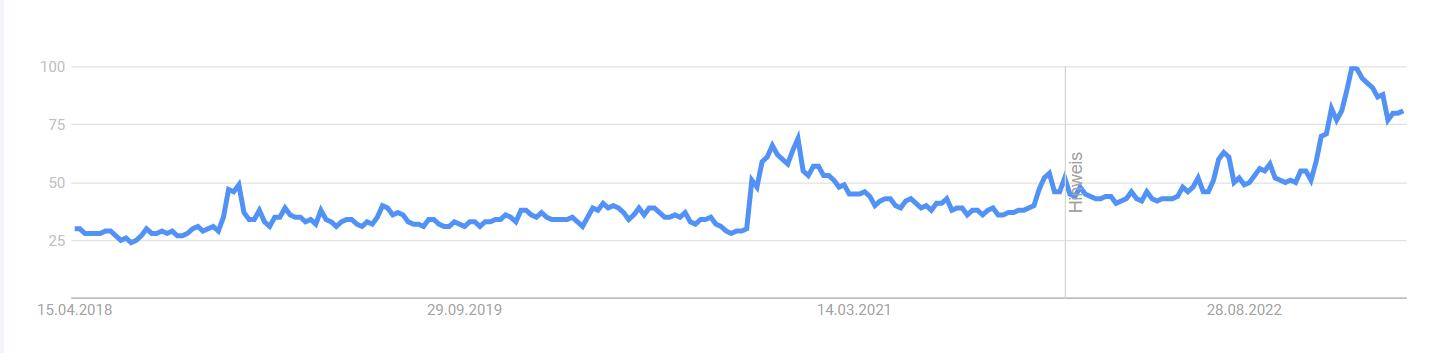
\includegraphics[width=160mm]{Schachentwicklung.jpg}
    \footnotesize\sffamily\textbf{Quelle:} \url{https://trends.google.de/}
  \caption{Relatives Suchinteresse des Wortes \textit{Chess} auf Google in den letzten 5 Jahren.}
  \label{fig:Schachinteresse}
\end{figure}
  
  \begin{figure}[ht]
\raggedleft
  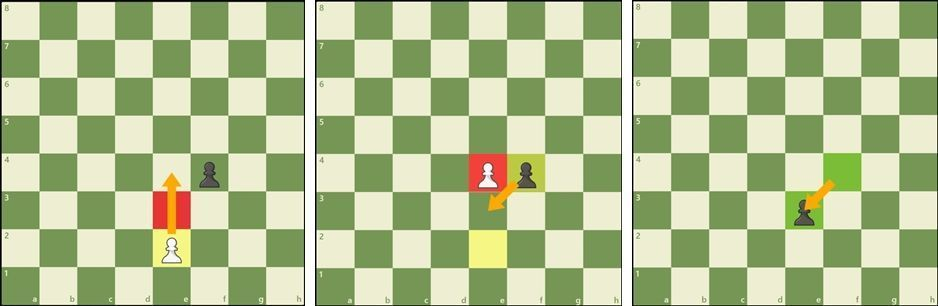
\includegraphics[width=160mm]{en-passant.jpeg}
    \footnotesize\sffamily\textbf{Quelle:} \url{https://www.chess.com/de/schachregeln}
  \caption{Die Zusatzregel \textit{en passant}}
  \label{fig:en-passant}
\end{figure}

  \begin{figure}[ht]
\centering
  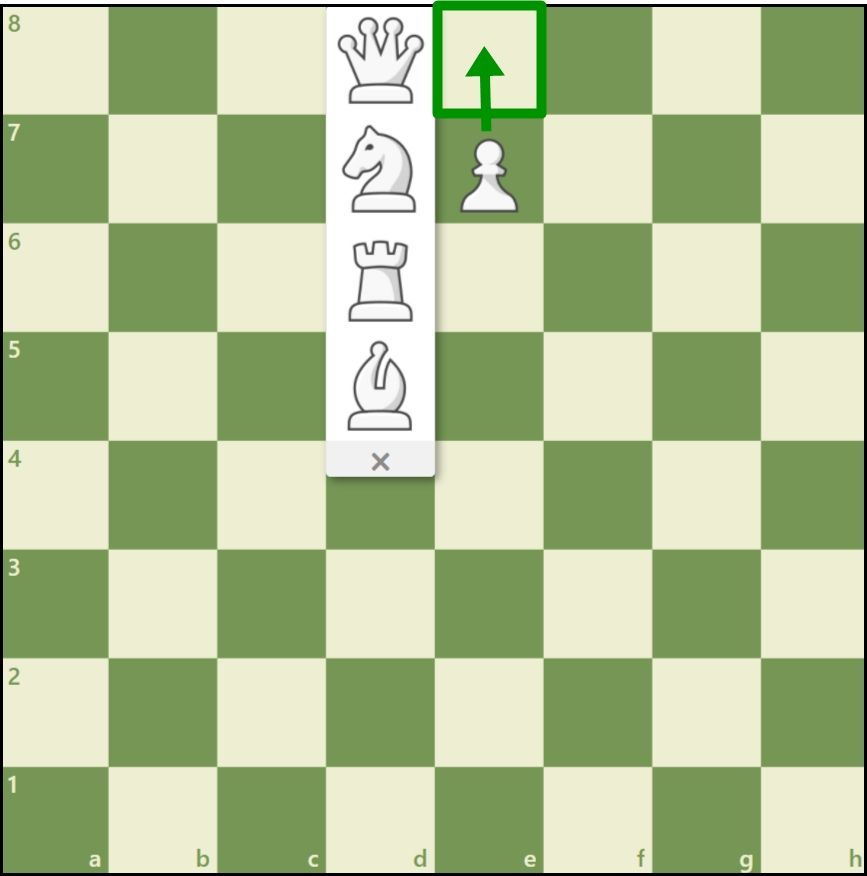
\includegraphics[height=80mm]{promotion.jpeg}
   
   
\raggedleft
    \footnotesize\sffamily\textbf{Quelle:} \url{https://www.chess.com/de/schachregeln}
  \caption{Die Zusatzregel \textit{Bauernumwandlung}}
  \label{fig:promotion}
\end{figure}

  \begin{figure}[ht]
\raggedleft
  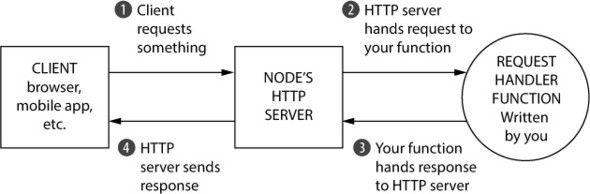
\includegraphics[width=160mm]{node-request.jpg}
    \footnotesize\sffamily\textbf{Quelle:} \cite{expressbook}
  \caption{Ablauf einer Anfrage an einen Node.js Server}
  \label{fig:node-request}
\end{figure}


  \begin{figure}[ht]
\raggedleft
  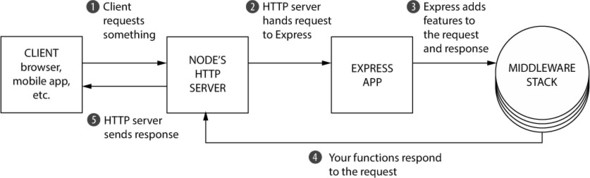
\includegraphics[width=160mm]{express-request.jpg}
    \footnotesize\sffamily\textbf{Quelle:} \cite{expressbook}
  \caption{Ablauf einer Anfrage an einen Node.js Server mit Express}
  \label{fig:express-request}
\end{figure}

  \begin{figure}[ht]
\raggedleft
  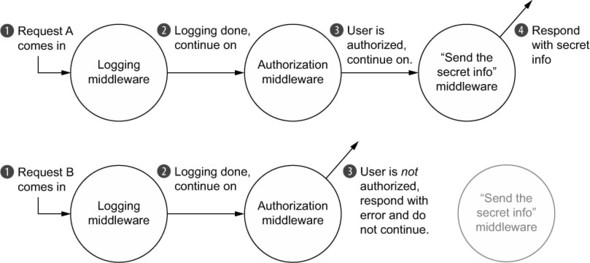
\includegraphics[width=160mm]{Middleware-Beispiel.jpg}
  
  \vspace{20mm}
  
  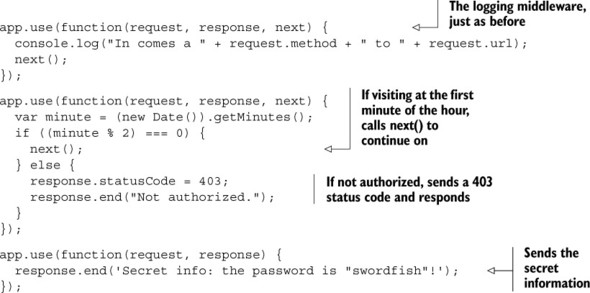
\includegraphics[width=160mm]{Middleware-Beispiel-2.jpg}
    \footnotesize\sffamily\textbf{Quelle:} \cite{expressbook}
  \caption{Beispiel der Nutzung von Middlewares}
  \label{fig:middleware-beispiel}
\end{figure}

  \begin{figure}[ht]
\raggedleft
  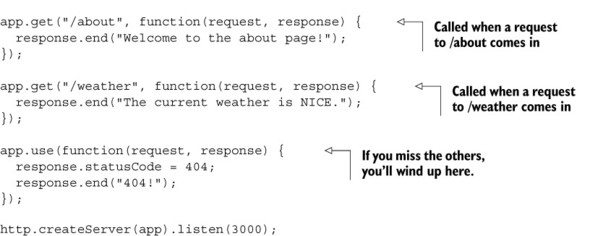
\includegraphics[width=160mm]{express-routing-example.jpg}
    \footnotesize\sffamily\textbf{Quelle:} \cite{expressbook}
  \caption{Beispiel der Nutzung von Routing}
  \label{fig:routing-beispiel}
\end{figure}

  \begin{figure}[ht]
\raggedleft
  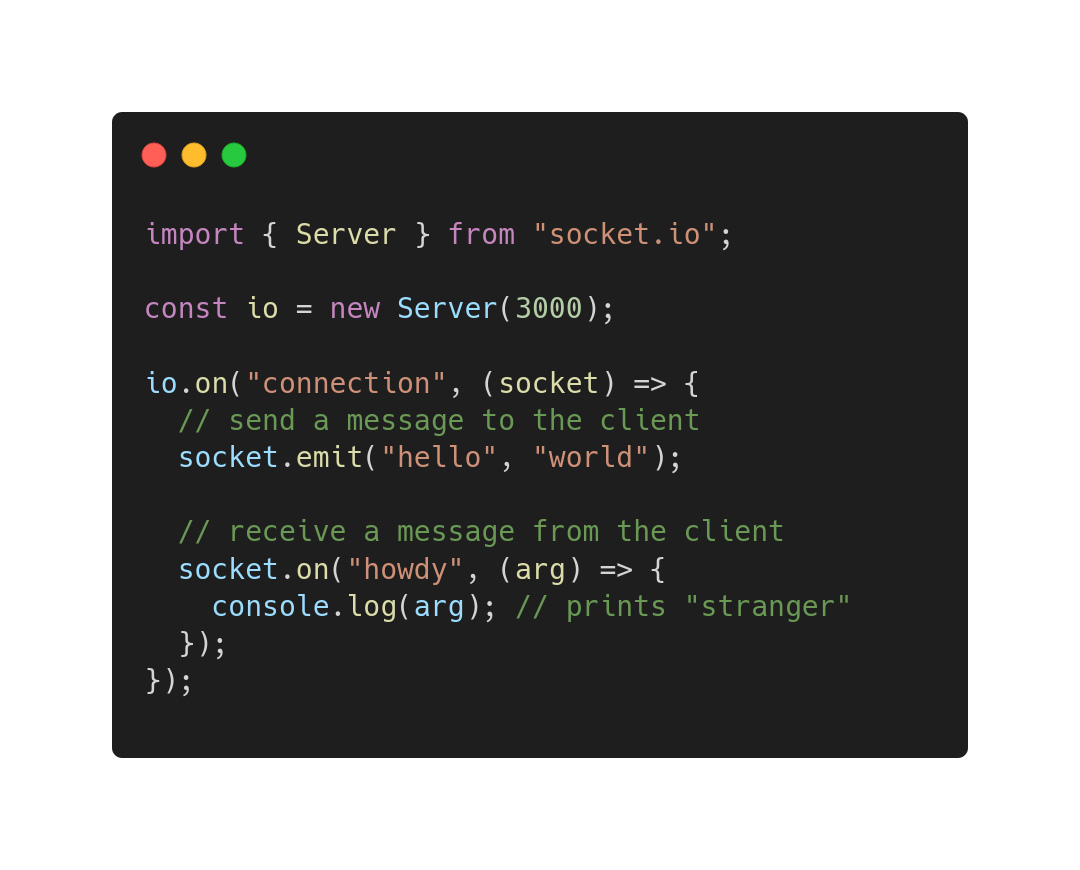
\includegraphics[width=70mm]{socket.io-server-beispiel.png}
  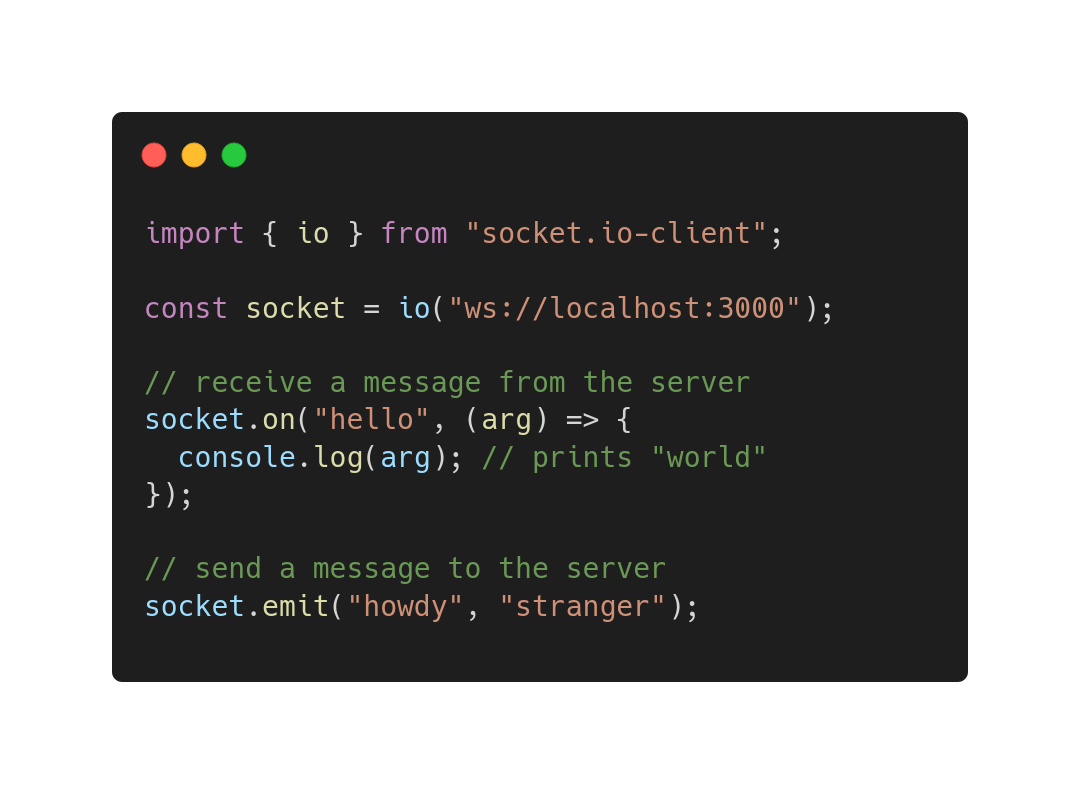
\includegraphics[width=70mm]{socket.io-client-beispiel.png}
    \footnotesize\sffamily\textbf{Quelle:} \cite{socketio}
  \caption{Simples Beispiel der Initialisierung einer socket.io Verbindung und das Senden und Empfangen von Events}
  \label{fig:socket.io-beispiel}
\end{figure}


\bibliography{Bibliography}

\end{document}

